\chapter{连续函数}

\section{函数的逐点连续和间断}

\subsection{基本概念}

类似于函数的极限, 函数的连续性有两种等价的定义: 

\begin{definition}{函数的连续性}
	设$f:E \to \R$, 若$E \ni a$是$E$的一个聚点, 我们称$f$在$a$点处\textit{连续}(continuous), 如果$\lim_{E \ni x \to a} f(x) = f(a)$. 等价地有: 
	
	-~~对于任意$\varepsilon >0$, 存在$\delta >0$使得$f(\mathring{N}_{\delta} (a)) \subseteq N_{\varepsilon} (f(a))$; 
	
	-~~对任意的数列$\{ x_n \}$, 若$\lim_{n \to \infty} x_n = a$, 则$\lim_{n \to \infty} f(x_n) = f(a)$. 
	
	\noindent
	特别地, 对于区间$[i,s) \subseteq E$, 若$\lim_{x \to s^-} f(x) = f(s)$, 称$f$在$s$处连续. 另一侧亦然. 
\end{definition}
\begin{remark}
	若将定义中的$a$拓广到$E$中的任意点, 按照第一种等价说法, 显然$a$为孤立点时$f$在$a$处连续. 
\end{remark}
\begin{remark}
	一种直观的写法是: $\lim_{x \to \infty} f(x_n) = f(\lim_{x \to \infty}x_n)$. 这是某种意义上的换序操作, 我们后面也会介绍不同的换序. 
\end{remark}

函数极限的Cauchy收敛准则依然适用: $f$在$a$连续当且仅当对任意$\varepsilon >0$, 存在$a$的邻域$N_{\delta} (a)$使得$\omega (f;N_{\delta} (a))<\varepsilon$. 特别地, 定义$\omega (f;a)= \lim_{\delta \to 0^+} \omega (f;N_{\delta} (a))$, 上式告诉我们$\omega (f;a)=0$, 即$f$在$a$处的振幅为$0$. 

这里给出一个有趣的事实: 我们知道$\omega (f;I)$可以写成$\sup_{x \in I} f(I) - \inf_{x \in I} f(I)$的形式, 那么$f$在$a$处连续当且仅当$$\lim_{\delta \to 0^+} \left( \sup_{x \in N_{\delta}(x_0)} f(x) \right)= \lim_{\delta \to 0^+} \left( \inf_{x \in N_{\delta}(x_0)} f(x) \right).$$
如果将上式中的邻域换成空心的, 这就分别是函数的上下极限(虽然我们没有讲过). 这时就要添加一个条件: 两侧极限都等于$f(x_0)$, 才能与上式等价. 

虽然连续是一个局部概念, 我们仍然愿意称$f$在$E$上连续当且仅当其在$E$的每个点上都连续, 这就是逐点连续的概念. 记$C(E)$为$E$上连续函数的全体. 

实际上, 初等函数都是连续的: 为此, 我们需要证明基本初等函数的连续性, 连续函数的四则运算(显然)和复合运算. 

\begin{example}
	证明$e^x$是$\R$上的连续函数. 
\end{example}
\begin{proof}
	待定$\delta >0$, 令$|x - x_0|<\delta$, 那么$$|e^x-e^{x_0}| \leq e^{x_0} \sum_{k=1}^{\infty} \frac{|x-x_0|^k}{k!} < e^{x_0} \sum_{k=1}^{\infty} \frac{\delta ^k}{k!} \leq \delta e^{x_0} \sum_{k=1}^{\infty} \frac{\delta ^{k-1}}{(k-1)!} = \delta e^{x_0+\delta}. $$
	所以我们让$\delta = \min (\frac{\varepsilon}{e^{x_0+1}}, 1)$即可得上式$<\varepsilon$. 
\end{proof}
\begin{remark}
	实际上, 利用上一章的指数函数构造可以直接证明$a^x$是$\R$上的连续函数. 
\end{remark}

\begin{example}
	证明$\sin x$是$\R$上的连续函数. 
\end{example}
\begin{proof}
	待定$\delta$, 令$|x-x_0|<\delta$, 那么$$|\sin x - \sin x_0| = 2\big| \cos \frac{x+x_0}{2} \sin \frac{x-x_0}{2} \big| \leq |x-x_0| < \delta .$$
	取$\delta = \varepsilon$即得. 
\end{proof}

\begin{example}
	定义Thomae函数如下: $$T(x) = \begin{cases}
 \frac{1}{q}  & \textit{ 若 } x=\frac{p}{q} \textit{ 且 } p\in \mathbb{Z}^*, q \in \mathbb{N}^*, \gcd(p,q)=1  \\
 0 & \textit{ 若 } x \in \R - \mathbb{Q} \cup \{ 0 \}
\end{cases}. $$
证明: $T$在有理数上不连续, 在无理数上连续. 
\end{example}
\begin{proof}
	只要证明, 对于给定的实数$x$, 若$\frac{p_n}{q_n} \to x$, 则$\frac{1}{q_n} \to 0$. 待定$\delta >0$使得$|\frac{p_n}{q_n} - x|<\delta$对足够大$n$成立, 我们有$$\frac{1}{|q_n|} < \frac{\min \{ |x-\delta|,|x+\delta| \}}{|p_n|} \leq \min \{ |x-\delta|,|x+\delta| \}.$$
	令$\delta = |x-\varepsilon |$即得. 
\end{proof}

\begin{proposition}{连续函数的复合运算}
	设$f \in C(I)$且$f$的值域在$J$中, $g \in C(J)$, 那么$gf \in C(I)$. 
\end{proposition}
\begin{proof}
	对于极限在$I$中的数列$\{ x_n \}$, $$\lim_{n\to \infty} g(f(x_n)) = g(\lim_{n\to \infty} f(x_n)) = g(f(\lim_{n\to \infty} x_n)).  $$
\end{proof}
\begin{remark}
	以上证明绕过了复合函数极限是否成立的验证. 
\end{remark}

连续函数的这种性质有助于我们进行极限的计算. 

\begin{example}
	求极限: $$\lim_{x\to 0} \frac{\ln (1+x)}{x}, \qquad \lim_{x\to 0} \frac{e^x-1}{x},\qquad \lim_{x\to 0} \frac{(1+x)^{\alpha}-1}{x}~(\alpha \neq 0). $$
\end{example}
\begin{solution}
	(1) 令$y=1/x$, 则$x \to 0$时$y \to \infty$. 那么, $$\lim_{x\to 0} \frac{\ln (1+x)}{x} = \lim_{x\to 0} \ln (1+x)^{1/x} = \lim_{y\to \infty} \ln \ssb{1+\frac{1}{y}}^y = \ln e = 1.$$
	
	(2) 这是(1)的显然推论. 
	
	(3) 由(1),(2)直接有$$\lim_{x\to 0} \frac{(1+x)^{\alpha}-1}{x} = \lim_{x\to 0} \frac{e^{\alpha \ln (1+x)}-1}{\alpha \ln (1+x)} \cdot \frac{\alpha \ln (1+x)}{x} = \alpha .$$
\end{solution}


\subsection{函数的间断点}

我们称$a \in E$是$f: E \to \R$的\textit{间断点}(point of discontinuity), 如果$f$在$a$处不连续. 下面对其进行分类: 

\begin{definition}{函数的间断点}
	设$f: E \to \R$, $a \in E$是$f$的间断点. 
	
	(1) 若极限$$\lim_{E \ni x \to a^-}=:f(a^-), \qquad \lim_{E \ni x \to a^+}=:f(a^+)$$都存在且至少有一个不等于$f(a)$, 称$a$为$f$的\textit{第一类间断点}(discontinuity of first kind); 
	
	(2) 若上述两个极限至少一个不存在, 称$a$为$f$的\textit{第二类间断点}(discontinuity of second kind). 
\end{definition}

称$a$为$f$的\textit{可去间断点}(removable discontinuity), 若存在$\tilde{f} \in C(E)$使得$\tilde{f} |_{E-a} = f |_{E-a}$. 显然, $a$为可去间断点当且仅当$\lim_{E \ni x \to a}f(x)$存在且不为$f(a)$: 此时我们只要将$f(a)$换成$\lim_{E \ni x \to a}f(x)$即可. 于是可以对第一类间断点进行进一步分类: 若$f(a^-) = f(a^+)$, $a$就是所谓可去间断点; 若不然, 称$a$是$f$的\textit{跳跃间断点}(jump discontinuity), 并称$|f(a^-) - f(a^+)|$为$f$在$a$处的\textit{跃度}(jump). 

\begin{lemma}{}\label{lem:djdnhjuuzoyzjixm}
	$I$是区间, $f:I \to \R$是$I$上的单调函数, 则对任意$x_0 \in I$, $f$在$x_0$处的左右极限均存在. 特别地, 设$f$单调不减, 那么$$\lim_{x \to x_0^-} f(x) = \sup_{x \in (-\infty,x_0) \cap I} f(x),\qquad \lim_{x \to x_0^+} f(x) = \inf_{x \in (x_0,+\infty) \cap I} f(x).$$
\end{lemma}
\begin{proof}
	这是定理\ref{thm:djdnhjuudejixm}的直接推论. 
\end{proof}

下方关于间断点的定理实际是在说: $f$在$I$中的大多数点上连续. 

\begin{theorem}{Froda}
	$I$是区间, $f:I \to \R$是$I$上的单调函数. 记$f$在$I$上间断点的集合为$D(f)$, 则$D(f)$是至多可数的. 
\end{theorem}
\begin{proof}
	不妨考虑$f$单调不减, 由引理可知对$x_0 \in D(f)$有$\lim_{x \to x_0^-} f(x) < \lim_{x \to x_0^+} f(x)$. 因此, $x_0$确定了一个开区间$I_{x_0}=(\lim_{x \to x_0^-} f(x) , \lim_{x \to x_0^+} f(x))$. 我们在$I_{x_0}$中选取一个有理数$q_{x_0}$, 下面证明映射$q_{\bigcdot}$是单射, 也就是说对$x_1,x_2 \in D(f)$, $I_{x_1} \cap I_{x_2} = \varnothing$: 不妨设$x_1<x_2$. 由引理可知$\lim_{x \to x_1^+} f(x) \leq \lim_{x \to x_2^-} f(x)$, 而$I_{x_1},I_{x_2}$均为开区间, 所以它们不交. 
	
	既然$q_{\bigcdot}$是单射, 那么$D(f)$是至多可数的. 
\end{proof}

下方的命题能促进对这一方法的进一步理解. 

\begin{proposition}{}
	设$f \in C([a,b])$且严格单调递增, 那么$f$是$[a,b] \to [f(a),f(b)]$的双射且其逆映射$f^{-1}:[f(a),f(b)] \to [a,b]$是连续且严格单调递增的. 
\end{proposition}
\begin{proof}
	容易证明$f^{-1}$是双射且严格单调递增. 下面证明其是连续的. 
	
	用反证法. 假设$f(x_0)=y_0 \in [f(a),f(b)]$是$f^{-1}$的一个间断点, 由引理\ref{lem:djdnhjuuzoyzjixm}知存在一个开区间$I_{y_0}=(x_1,x_2)$, 其中$x_1=\sup_{z<y_0}f^{-1}(z),x_2=\inf_{z>y_0}f^{-1}(z)$, 使得$y_0 \in I_{y_0}$. 显然$x_1 \leq x_0 \leq x_2$. 但对于$y<y_0$均有$f^{-1}(y)<x_1$, 对$y>y_0$均有$f^{-1}(y)>x_2$, 意味着$(x_1,x_2)-\{ x_0 \} \nsubseteq [a,b]$, 矛盾. 
\end{proof}

我们再做一个相关的练习: 

\begin{proposition}{}
	设$f \in C([a,b])$, 则$f$是单射当且仅当$f$在$[a,b]$上严格单调. 
\end{proposition}
\begin{proof}
	充分性显然. 必要性: 不妨$f(a)<f(b)$. 假设$a \leq x_1 < x_2 \leq b$满足$f(b) \geq f(x_1) \geq f(x_2) \geq f(a)$, 那么$[f(a),f(x_1)] = f([a,x_1]), [f(x_2),f(b)] = f([x_2,b])$, 从而存在$z_1 \in [a,x_1],z_2 \in [x_2,b]$使得$f(z_1)=f(z_2) \in [f(x_2),f(x_1)]$, 与单射性矛盾. 
\end{proof}

\section{闭区间上连续函数的性质}

\begin{theorem}{Bolzano-Cauchy中值定理}
	设$f:[a,b] \to \R$是连续函数. 若$f(a) \cdot f(b) <0$, 则存在$c \in (a,b)$使得$f(c)=0$. 特别地, 若$f(a) \neq f(b)$, 则对任意$y \in [f(a),f(b)]$, 存在$c \in (a,b)$使得$f(c)=y$. 
\end{theorem}
\begin{remark}
	我们可以将$[a,b]$拓广到所谓“连通的”集合上. 
\end{remark}
\begin{proof}
	\underline{\textbf{证法一}}~~令$I_0=[a,b]$, 不妨假设$f(\frac{a+b}{2}) \neq 0$, 若$f(\frac{a+b}{2}) \cdot f(a)<0$则取$I_1=[a,\frac{a+b}{2}]$, 反之则取$I_1=[\frac{a+b}{2},b]$. 类似地进行构造, 我们最后得到闭区间套$I_0 \supseteq \cdots \supseteq I_n \supseteq \cdots$且$|I_n|\to 0,n \to \infty$. 从而, 存在唯一的$c \in \bigcap_{n\geq 0}I_n$. 若$f(c) \neq 0$, 不妨设其为正, 在函数连续性的定义中选择$\varepsilon = \frac{f(c)}{2}$, 容易说明存在$c$的一个邻域使得$f$在上面为正, 取更小的邻域即得矛盾. 
	
	\underline{\textbf{证法二}}~~同上构造闭区间套, 我们取$I_n$的左右端点构成数列$\{ x_n \}$和$\{ y_n \}$, 利用函数的连续性可得$\lim_{n\to \infty} x_n = f(c) \leq 0$, $\lim_{n\to \infty} y_n = f(c) \geq 0$, 故$f(c)=0$. 
\end{proof}

利用中值定理, 我们可以证明压缩映射原理在$\R$上的特殊情况: 

\begin{proposition}{($\R$上的)压缩映射原理}
	设$f:\R \to \R$是压缩映射, 即存在常数$0 < c < 1$使得对任意$x,y \in \R$都有$|f(x)-f(y)| \leq c|x-y|$. 那么, $f$必有唯一的不动点, 即存在唯一的$x_0 \in \R$使得$f(x_0)=x_0$. 
\end{proposition}
\begin{proof}
	令$F(x) = f(x) - x$, 任取$x<y$可得$F(x)-F(y) = (f(x)-f(y)) - (x-y) \geq (1-c)(y-x) >0$, 从而$F(x)$在$\R$上严格单调递减. 
	
	任取$M>0$, 由于$f(x) \leq f(0)+cx$, 只要取$x > \frac{M+f(0)}{1-c}$就有$f(x)-x<-M$, 从而说明$F(x) \to -\infty ,x \to +\infty$, 同理可得$F(x) \to +\infty ,x \to -\infty$. 又显然$f$连续, 所以$F$连续, 从而$F$在$\R$上存在唯一零点. 
\end{proof}


\begin{theorem}{Weierstrass最大值定理}
	设$f \in C([a,b])$, 那么$f$有界, 且存在$x_1,x_2 \in [a,b]$使得$f(x_1) = \inf_{x \in [a,b]} f(x), f(x_2) = \sup_{x \in [a,b]}f(x)$. 
\end{theorem}
\begin{remark}
	我们可以将$[a,b]$拓广到所谓“紧的”集合上. 
\end{remark}
\begin{proof}
	(1) \underline{\textbf{证法一}}~~用反证法. 假设存在数列$\{ x_n \} \subseteq I$使得$f(x_n) \to \infty$. 通过选取$\{ x_n \}$的子列我们不妨让$x_n \to x$, 显然$x \in I$, 所以$f(x_n) \to f(x)$, 矛盾. 
	
	\underline{\textbf{证法二}}~~显然对任意$x_0 \in I$, 存在$x_0$的一个邻域$N(x_0)$使得$f$在$N(x_0)$上有界. 由于$\bigcup_{x \in I} N(x)$构成$I$的一个开覆盖, 可取其中的有限个, 设为$N(x_1), \cdots ,N(x_n)$, 而$f$在这些邻域上均有界, 故在$[a,b]$上亦有界. 
	
	(2) \underline{\textbf{证法一}}~~以上确界为例. 设$M=\sup_{x \in I}f(x)$, 假设$M-f(x)$在$I$上处处不为零, 但我们注意到其可以无限接近零, 那么连续函数$\frac{1}{M-f(x)}$是无界的, 与(1)矛盾. 
	
	\underline{\textbf{证法二}}~~由上确界的定义可知, 对任意的$n$都存在$x_n \in I$使得$M-\frac{1}{n} < f(x_n) \leq M$, 通过选取$\{x_n\}$的子列我们不妨让$x_n \to x \in I$, 从而在上式的两侧取极限得$f(x)=M$. 
	
	在证明中, 请注意子列的极限在$I$中是由于数列极限对不严格不等号的保序性. 
\end{proof}

下面介绍所谓一致连续性. 

\begin{definition}{函数的一致连续性}
	设$f:E \to \R$, 称$f$在$E$上\textit{一致连续}(uniformly continuous), 如果对任意$\varepsilon >0$都存在$\delta >0$使得对任意$x,y \in E$, 只要$|x-y|<\delta$就有$|f(x)-f(y)|<\varepsilon$. 
\end{definition}
\begin{remark}
	有些书上将一致连续性的定义缩小到区间上, 这样做是合理的, 因为可以证明: 若$f$在有限个区间上分别一致连续, 则在它们的并集上也一致连续, 具体参考定理4.4. 我们接下来也会专注于某个区间上的函数的一致连续性. 
\end{remark}

\begin{example}
	证明$f(x)=\frac{1}{x}$在$(0,+\infty)$上并非一致连续, 而在$(c ,+\infty ), c >0$上一致连续. 
\end{example}
\begin{proof}
	(1) 假设存在$\delta >0$符合要求, 任取$\varepsilon >0$, 由于$$\varepsilon > |\frac{1}{x}-\frac{1}{y}| = \frac{|x-y|}{xy},$$
	所以$\delta <xy\varepsilon$. 由$x,y$选取的任意性可知$\delta =0$, 矛盾. 
	
	(2) 取$\delta = c^2\varepsilon$即可. 
\end{proof}

这个例子很清晰地展示了一致连续性的要求: 不能出现增长率无穷大的情况. 实际上这种(充分的)判别方法就是Lipschitz方法: 

\begin{proposition}{Lipschitz}
	设区间$I$, $f \in C(I)$. 若存在常数$L$使得对任意$x,y \in I$都有$|f(x)-f(y)| \leq L|x-y|$, 那么$f$一致连续. 
\end{proposition}

我们也可以选择用数列极限来刻画(区间上的)一致连续性: 

\begin{proposition}{}
	设$f:I \to \R$, 其中$I$是区间. $f$在$I$上一致连续当且仅当对任意数列$\{ x_n \},\{ y_n \} \subseteq I$, 只要$x_n- y_n \to 0$, 就有$\lim_{n\to \infty} (f(x_n)-f(y_n))=0$. 
\end{proposition}
\begin{proof}
	必要性是显然的. 充分性: 假设$f$在$I$上并非一致连续, 则存在$\varepsilon >0$使得对任意$n$都存在$x_n,y_n$使得$|x_n-y_n|<\frac{1}{n}, |f(x_n)-f(y_n)| \geq \varepsilon$, 即说明$f(x_n) - f(y_n) \nrightarrow 0$, 矛盾. 
\end{proof}

\begin{example}
	证明$f(x)=x^2$在$[0,+\infty)$上并非一致连续. 
\end{example}
\begin{proof}
	选取$x_n=n+\frac{1}{n},y_n=n$, 那么$x_n-y_n \to 0$, 但是$f(x_n)-f(y_n)=2+\frac{1}{n^2} \to 2$, 故$f$在$[0,+\infty)$上并非一致连续. 
\end{proof}

上面的例子指出: 在某个区间上无界(当然只能是开区间)的逐点连续函数不一定一致连续. 反过来, 就是所谓Cantor-Heine定理: 

\begin{theorem}{Cantor-Heine的一致连续性定理}
	若$f \in C([a,b])$, 则$f$一致连续. 
\end{theorem}
\begin{remark}
	类似于上一个定理, 我们可以将$[a,b]$拓广到所谓“紧的”集合上. 
\end{remark}
\begin{proof}
	\underline{\textbf{证法一}}~~任取$\varepsilon >0$, 显然对任意$x_0 \in I$, 存在$x_0$的一个邻域$N_{\delta(x_0)}(x_0)$使得$f$在$N(x_0)$上的振幅$\omega (f;N_{\delta(x_0)}(x_0)) <\varepsilon$. 由于$\bigcup_{x \in I} N_{\delta(x_0)}(x_0)$构成$I$的一个开覆盖, 可取其中的有限个使得它们仍然构成一个开覆盖, 设为$N_{\delta (x_1)}(x_1), \cdots ,N_{\delta (x_n)}(x_n)$. 我们选取$\delta _0 = \frac{1}{2}\min \{ \delta (x_1),\cdots ,\delta (x_n) \}$, 考虑$|x-y|<\delta _0$, 显然存在$\ell$使得$x,y \in N_{\delta (x_{\ell})}(x_{\ell})$, 所以立得$|f(x)-f(y)|<\varepsilon$. 
	
	\underline{\textbf{证法二}}~~设若不然, 则存在$\varepsilon >0$使得对任意$n >0$, 存在$|x_n-y_n|<1/n$且$|f(x_n)-f(y_n)| \geq \varepsilon$. 通过选取$\{ x_n \}$的子列, 不妨设其极限为$x \in I$, 进而显然有$y_n \to x$. 由于$f$在$x$处连续, 可知$\lim_{n\to \infty} f(x_n) = \lim_{n\to \infty} f(y_n) = x$, 得到矛盾. 
\end{proof}

对于开区间我们也有一致连续的充要条件, $f(x)=\frac{1}{x}$的例子就是一个印证. 

\begin{proposition}{}
	设$f \in C((a,b))$, 其中$a,b$可以为$\infty$. 则$f$一致连续当且仅当$f(a^+),f(b^-)$存在(且有限). 
\end{proposition}
\begin{proof}
	必要性: 任取$\varepsilon >0$则存在$\delta >0$使得任意的$|x-y|<\delta$都有$|f(x)-f(y)|<\delta$, 那么对$|x-a|<\delta /2, |y-a|<\delta /2$都有$|f(x)-f(y)|<\delta$, 这说明$f(a^+)$存在. 另一侧是类似的. 
	
	充分性: 只需要将$f$补为$[a,b]$上的连续函数$$F(x)=\begin{cases}
 f(x), & a<x<b \\
 f(a^+) & x=a \\
 f(b^-) & x=b
\end{cases}.$$
\end{proof}

最后介绍一个刻画一致连续性的优雅命题: 

\begin{proposition}{}
	设$f:E \to \R$, 其中$E$是长度有限的区间, 则$f$在$E$上一致连续当且仅当对所有Cauchy列$\{ x_n \} \subseteq E$, $\{ f(x_n) \}$仍然是Cauchy列. 
\end{proposition}
\begin{proof}
	必要性显然. 充分性: 假设$f$并非一致连续, 即存在$\varepsilon >0$使任意$\delta >0$都有$|x-y|<\delta \Rightarrow |f(x)-f(y)| \geq \varepsilon$. 特别地, 取$\delta = 1/n$, 构造数列$\{ x_n \},\{ y_n \}$使得$|x_n-y_n|<1/n$. 由于$E$有界, $\{ x_n \}$和$\{ y_n \}$都存在收敛子列, 将两个收敛子列的点交错排序得到Cauchy列$\{ z_n \}$, 但是$\{ f(z_n) \}$不是Cauchy列, 矛盾. 
\end{proof}

关于一致连续函数的运算, 设$f,g$分别在区间$I$上一致连续, 显然有$f+g$在$I$上一致连续. 由于乘法需要用到有界性来约束, 自然会考虑: 

\begin{proposition}{}
	设$f,g$在有限区间$I$上一致连续, 则$f \cdot g$在$I$上一致连续. 
\end{proposition}
\begin{proof}
	问题的关键是在于证明: 若$f$在$I$上一致连续, 则有界. 当$I$是闭区间时结论显然; 当$I$有至少一边是开的时, 利用命题4.6的方法将其补全为闭区间上的函数, 由于$f$在$I$两端的极限均为实数, 这样的补全是合理的, 从而证明了结论. 
\end{proof}

\newpage
\subsection*{一些习题 ~~\small 对应原书4.2习题}
















\newpage
\section{度量空间及其完备化}

\subsection{度量空间的基本概念}

\begin{definition}{度量空间}
	设集合$X$. 若存在$d:X \times X \to \R _{\geq 0}$满足: 
	
	a) 正定性: 对任意$x,y \in X$, $d(x,y)\geq 0$且取等号当且仅当$x=y$; 
	
	b) 可交换性: 对任意$x,y \in X$, $d(x,y)=d(y,x)$; 
	
	c) 三角不等式: 对任意$x,y,z \in X$, $d(x,z) \leq d(x,y)+d(y,z)$. 
	
	\noindent
	则称$(X,d)$是一个\textit{度量空间}(metric space), $d$是该度量空间上的\textit{距离函数}(metric function). 
\end{definition}
\begin{remark}
	需要注意, 度量空间都是建立在$\R$上的. 
\end{remark}

例如, $\R ^n$上可以定义三种距离函数: $$d_1(x,y) := \sum_{j=1}^n |x_j-y_j|,\qquad d_n(x,y) := \sqrt[n]{\sum_{j=1}^n |x_j-y_j|^n},\qquad d_{\infty}(x,y) := \sup_{1 \leq j \leq n}|x_j-y_j|. $$
由基本的代数不等式技巧可以验证它们确实是距离函数. 

接着我们定义度量空间$(X,d)$的\textit{子空间}$(Y,d_Y)$, 如果$Y \subseteq X$并且$d_Y = d|_{Y \times Y}$. 

\begin{definition}{度量空间中的极限}
	设点列$\{ x_n \}$, 若存在$x \in X$使得对任意的$\varepsilon >0$都存在正整数$N$, 使得对任意正整数$n\geq N$都有$d(x_n,x)<\varepsilon$, 就称$\{ x_n \}$的\textit{极限}(limit)是$x$. 
\end{definition}
\begin{remark}
	$\R$上数列极限的绝大多数性质都可以用同样的方法在度量空间中得到证明, 因此后文直接假设这些性质已经证过了. 
\end{remark}

我们可以在同一个集合$X$上定义不同的距离函数$d_1,d_2$. 称$d_1,d_2$是等价的, 如果存在正的常数$c_1,c_2$使得$$\forall x,y \in X, c_1d_1(x,y) \leq d_2(x,y) \leq c_2d_1(x,y).$$
容易证明, $x_n \stackrel{d_1}{\longrightarrow} x$和$x_n \stackrel{d_2}{\longrightarrow} x$是等价的. 因此只需考虑一种(好算)的距离即可. 

我们称$\{ x_n \}$为一个\textit{Cauchy列}, 如果对任意的$\varepsilon >0$, 都存在$N$使得任意$m,n \geq N$都有$d(x_m,x_n)$. 有关度量空间很重要的一个主题是, 其是否是\textit{完备}的, 这里我们定义\textit{完备}就是指所有Cauchy列都收敛. 

类似于$\mathbb{Q}$在$\R$中的稠密性, 对于度量空间$(X,d)$和$Y \subseteq X$, 称$Y$在$X$中\textit{稠密}(dense), 如果对任意$x \in X, \varepsilon >0$都存在$y \in Y$使得$d(y,x) < \varepsilon$. 

\begin{definition}{赋范向量空间, 范数}
	设$V$是$\R$(或者$\C$)上的向量空间. 若存在$\| \bigcdot \|:V \to \R _{\geq 0}$满足: 
	
	a) 齐次性: 对任意$x \in V, \lambda \in \R$, $\| \lambda x \|=|\lambda | \| x \|$; 
	
	b) 非退化性: 对任意$x \in V$, $\| x \|=0$当且仅当$x=0$; 
	
	c) 三角不等式: 对任意$x,y \in V$, $\| x+y \| \leq \| x \|+\| y \|$. 
	
	\noindent
	则称$(V,\| \bigcdot \| )$是一个\textit{赋范向量空间}(normed vector space), $\| \bigcdot \|$是该空间上的\textit{范数}(norm). 
\end{definition}
\begin{remark}
	如果不加解释, 我们通过定义$(V,d(x,y)=\| x-y \|)$将赋范向量空间看作度量空间. 
\end{remark}

例如, $\R ^n$上可以定义三种范数: $$\| x \|_1 := \sum_{j=1}^n |x_j|,\qquad \| x \|_n := \sqrt[n]{\sum_{j=1}^n |x_j|^n},\qquad \| x \|_{\infty} := \sup_{1 \leq j \leq n}|x_j|. $$

同样地可以定义赋范向量空间上的等价范数. 事实上, 对于有限维赋范向量空间, 上面所有的范数都是等价的. 

\begin{proposition}{}
	$n$维向量空间$V$上的所有范数都等价. 
\end{proposition}
\begin{proof}
	在该命题的证明中需要用到$\R ^n$上函数的连续性相关命题, 我们先承认这些命题正确. 
\end{proof}

如果一个赋范向量空间是完备的, 我们通常称其为Banach空间. 

赋范向量空间较于一般的度量空间的优势在于: 它对于加法和标量乘法是封闭的. 也就是说我们会有显然的性质$\lim_{n\to \infty} (x_n+y_n) = \lim_{n\to \infty} x_n + \lim_{n\to \infty} y_n$和$\lim_{n\to \infty} \lambda x_n = \lambda \lim_{n\to \infty} x_n$. 特别地, 考虑矩阵的空间$(\R ^{n\times n},\| \bigcdot \|)$, 其中$$\| A \| := \sup_{1 \leq i,j \leq n} |A_{ij}|,$$
我们希望得到$\lim_{n\to \infty} (x_n \cdot y_n) = \lim_{n\to \infty} x_n \cdot \lim_{n\to \infty} y_n$. 
\begin{proof}
	问题的关键在于, 在$\R$上$|xy|=|x||y|$, 而在矩阵空间中这一点未必成立. 不过我们可以有$$\| A \cdot B \| = \sup_{1 \leq i,j \leq n} |\sum_{k=1}^{n}A_{ik}B_{kj}| \leq \sum_{k=1}^n (\sup_{1 \leq i,j \leq n} |A_{ij}|)(\sup_{1 \leq i,j \leq n} |B_{ij}|) = n\| A \| \| B \|,$$
	也就是说存在一个常数$C$使得$\| x\cdot y \| \leq C\| x \| \| y \|$. 于是我们有$$d(x_n \cdot y_n,x \cdot y) \leq \| (x_n-x)y_n \| 
		+ \| x(y_n-y) \| \leq C(\| x_n-x \| \| y_n \| 
		+ \| x \| \| y_n-y \|),$$
	接下来的控制就是熟知的了. 
\end{proof}

\subsection{度量空间的完备化}

下面进行一项有趣的操作: 将任何一个度量空间$(X,d)$完备化. 直观上来讲, 我们希望$(X,d)$的完备化空间$(\overline{X},\overline{d})$是最小的. 以$\mathbb{Q}$为例, 我们可以将其认作$\tilde{\mathbb{Q}}=\{ (x,0):x \in \mathbb{Q} \}$, 并将$\R$认作$\tilde{\R}=\{ (x,0):x \in \R \}$. 注意到$\tilde{\mathbb{Q}}$在$\tilde{\R}$中稠密, 但在$\R ^2$中不稠密. 因此我们可以通过稠密性来确定这一最小性:

\begin{definition}{完备化空间}
	设度量空间$(X,d)$是$(\overline{X},\overline{d})$的子空间, 称其是$(X,d)$的\textit{完备化空间}(completion), 如果$X$在$\overline{X}$中稠密. 
\end{definition}

当然要证明度量空间的完备化空间是唯一的, 或者至少在某种等价条件下是唯一的. 这种等价条件就是所谓等距: 

\begin{definition}{等距的度量空间}
	称$(X_1,d_1)$与$(X_2,d_2)$\textit{等距}(isometric), 如果存在\textit{等距映射}(isometry)$f:X_1 \to X_2$满足: 
	
	a) $f$是双射; \qquad b) 对任意的$x,y \in X_1$都有$d_2(f(x),f(y))=d_1(x,y)$. 
\end{definition}

\begin{proposition}{}
	若$(X_1,d_1),(X_2,d_2)$均为$(X,d)$的完备化空间, 则它们是等距的. 
\end{proposition}
\begin{proof}
	如下构造等距映射$f$: 若$x \in X$则$f(x) = x$; 若$x_1 \in X_1-X$, 由$X$在$X_1$中稠密可知存在$\{ z_n \} \subseteq X$使得$z_n \stackrel{d_1}{\longrightarrow} x_1$, 因此$\{ z_n \}$在$d_1$下是Cauchy列. 由于在$X$上$d,d_1,d_2$是一样的, 所以$\{ z_n \}$在$d_2$下也是Cauchy列, 记$z_n \stackrel{d_1}{\longrightarrow} x_2$, 并令$f(x_1)=x_2$. 显然$f$是单射, 并且将这个过程反过来就得到$f$是满射. 
	
	下面证明$f$是等距映射: 对于$x,x'$, 选择$\{ z_n \},\{ z'_n \} \subseteq X$使得它们在$d_1$下极限分别为$x,x'$. 注意到$$|d_1(z_n,z'_n)-d_1(x,x')| \leq d_1(z_n,x) + d_1(z'_n,x'),$$
	因此$$d_1(x,x') = \lim_{n\to \infty} d_1(z_n,z'_n) = \lim_{n\to \infty} d_2(z_n,z'_n) = d_2(f(x),f(x')).$$
\end{proof}

现在我们考虑构造完备化空间的一般方法. 特别地, 从上方命题的证明中可以猜到$\overline{X}$应该与Cauchy列有关. 

\begin{definition}{度量空间的完备化}
	设度量空间$(X,d)$, 下面定义其完备化空间$(\overline{X},\overline{d})$. 
	
	\begin{itemize}
		\item 令$\mathcal{C} = \{ \{ x_n \} \subseteq X: \textit{$\{ x_n \}$是Cauchy列} \}$, 定义$\mathcal{C}$上的等价关系$\sim$: $$\{ x_n \} \sim \{ y_n \} \quad \Leftrightarrow \quad \lim_{n\to \infty} d(x_n,y_n)=0.$$
		取$\overline{X} = \mathcal{C} / \sim$. 
		\item 定义$\overline{X}$上的距离函数$\overline{d}$: $$\overline{d} : \overline{X}^2 \to \R,\quad ([\{ x_n \}], [\{ y_n \}]) \mapsto \lim_{n\to \infty} d(x_n,y_n). $$
	\end{itemize}
\end{definition}
\begin{remark}
	关于距离函数$\overline{d}$良定义性的验证分为两部分: $\lim_{n\to \infty} d(x_n,y_n)$总是存在且与代表元选取无关. 
	
	(1) 注意到$$|d(x_n,y_n) - d(x_m,y_m)| \leq |d(x_n,y_n)-d(x_m,y_n)|+|d(x_m,y_n)-d(x_m,y_m)| \leq d(x_n,x_m)+d(y_n,y_m), $$
	容易得到$d(x_n,y_n)$是Cauchy列, 所以收敛. 
	
	(2) 若$\{ x'_n \} \sim \{ x_n \}, \{ y'_n \} \sim \{ y_n \}$, 由于$$|d(x_n,y_n) - d(x'_n,y'_n)| \leq |d(x_n,y_n) - d(x'_n,y_n)| + |d(x'_n,y_n) - d(x'_n,y'_n)| \leq d(x_n,x'_n) + d(y_n,y'_n), $$
	可得$\lim_{n\to \infty} d(x_n,y_n) = \lim_{n\to \infty} d(x'_n,y'_n)$. 
\end{remark}

验证$\overline{d}$是距离函数比较容易. 

现在, 我们思考怎样将$X$视作$\overline{X}$的子空间. 具体来说, 我们定义嵌入映射$$\iota : X \to \overline{X},\quad x \mapsto [\{ x_n=x \}]. $$
容易验证, 若$x\neq y$则$\iota (x) \neq \iota (y)$, 从而$\iota$是单射, 符合嵌入映射的要求. 另一方面, $\iota$是等距映射, 即$\overline{d} (\iota (x),\iota (y)) = d(x,y)$. 从而, 我们可以证明$X$在$\overline{X}$中稠密: 对于$[\{ x_n \}] \in \overline{X}$, 和任意的$\varepsilon >0$, 存在$N$使得任意$n>N$有$d(x_n,x_N)<\varepsilon$, 从而$\overline{d} (\iota (x_N),[\{ x_n \}]) < \varepsilon$. 

最后, 我们说明$(\overline{X}, \overline{d})$是完备的. 基本的思路类似于定理\ref{pro:hjuucauchy}的证法一, 即我们需要从Cauchy序列中构造出一个极限来. 

\begin{proof}
	设$\overline{x}^{(n)} \in \overline{X}$, 则对每个$\overline{x}^{(n)}$都存在$x_n \in X$使得$\overline{d}(\overline{x}^{(n)},\iota (x_n))<1/n$. 容易验证$\{ x_n \}$是Cauchy列, 因为对$m \neq n$有$$d(x_m,x_n) \leq \overline{d} (\iota (x_m), \overline{x}^{(m)}) + \overline{d} (\overline{x}^{(m)}, \overline{x}^{(n)}) + \overline{d} (\overline{x}^{(n)}, \iota (x_n)) \leq \frac{1}{m} + \frac{1}{n} + \overline{d} (\overline{x}^{(m)}, \overline{x}^{(n)}). $$
	设$\overline{x} = [\{ x_n \}]$. 下面说明, $\{ \overline{x}^{(n)} \}$的极限为$\overline{x}$. 其实只需计算$$\overline{d} (\overline{x}^{(n)} , \overline{x}) \leq \overline{d}(\overline{x}^{(n)},\iota (x_n)) + \overline{d}(\iota (x_n),\overline{x}) < \frac{1}{n} + \lim_{m\to \infty} d(x_n,x_m). $$
\end{proof}

需要注意的是, 度量空间的完备化针对距离函数来说是唯一的, 但我们可以选择不同的距离函数构造完备化空间. 例如, 利用Euclid度量$d(x-y)=|x-y|$将$\mathbb{Q}$完备化得到$\R$, 而利用$p$进绝对值$d_p(x,y) = p^{-v_p(x-y)}$将$\mathbb{Q}$完备化得到的不是$\R$. 

\subsection{压缩映射原理}



\newpage
\section{拓扑空间的基本概念}

\subsection{$\R$上的通常拓扑}

我们先将邻域的概念延拓一下并使用新的记号: 度量空间$(X,d)$上, 所谓以$x_0$为圆心, $\varepsilon$为半径的开球$B(x_0,\varepsilon)$, 定义为$\{ x \in X:d(x,x_0)<\varepsilon \}$. 

\begin{definition}{$\R$上的开集}
	设$U \subseteq \R$, 称$U$是$\R$上的一个\textit{开集}(open set), 若对任意$x \in U$都存在$\varepsilon >0$使得$B(x,\varepsilon) \subseteq U$. 
\end{definition}
\begin{remark}
	等价地, 让$x$遍历$U$可以得到开集的另一个定义: $U=\bigcup_{\alpha \in A} I_{\alpha}$, 其中$I_{\alpha}$是开区间, $A$是指标集. 
\end{remark}

一些开集的例子是: $\R$, $\varnothing$, 任意开区间, 任意开区间的并集. 一般地, 我们有如下的命题: 

\begin{proposition}{$\R$上开集的性质}
	设$\tau$表示$\R$上开集的全体. 
	\begin{itemize}
		\item $\R \in \tau$, $\varnothing \in \tau$; 
		\item $\bigcup_{\alpha \in A} U_{\alpha} \in \tau$, 其中$U_{\alpha}$是开集, $A$是指标集; 
		\item $\bigcap_{1 \leq i \leq n} U_i \in \tau$, 其中$U_i(i=1,\cdots ,n)$是开集. 
	\end{itemize}
\end{proposition}
\begin{remark}
	容易举出无限个开集的交集不是开集的例子: 设$I_n=(1-1/n,1+1/n)$, 则$\bigcap_{n\geq 1}I_n = \{ 1 \}$. 
\end{remark}
\begin{proof}
	前两条是显然的. 第三条: 任取$x \in \bigcap_{1 \leq i \leq n} U_i$, 对每个$i$都存在开区间$I_i \subseteq U_i$使得$x \in I_i$, 从而$x \in \bigcap_{1 \leq i \leq n} I_i \subseteq \bigcap_{1 \leq i \leq n} U_i$. 
\end{proof}

关于开集, 很自然地会有如下想法: 

\begin{proposition}{}
	设$U \subseteq \R$是开集, 则可将$U$拆分为可数个两两不交的开区间的并. 
\end{proposition}
\begin{remark}
	这是$\R$上的特殊性质, 无法推广. 
\end{remark}
\begin{proof}
	问题的关键是在于: 对每个$x \in U$需要找到一个最大的包含$x$的开区间$I_x$, 那么对于$x, y\in U$, 要么$I_x = I_y$, 要么$I_x \cap I_y = \varnothing$(否则, 存在$z \in I_x \cap I_y$, 所以$I_z = I_x = I_y$), 从而类似于Froda定理可以得到结论. 
	
	\underline{\textbf{证法一}}~~对于$x \in U$, 按如下方式构造$I_x$: 取最大的$\varepsilon \in \R \cup \{ +\infty \}$使得$X_0 = B(x,\varepsilon) \subseteq U$. 递归地定义$X_{n+1} = \bigcup_{x' \in X_n} B(x',\varepsilon _{x'})$, 其中$\varepsilon _{x'}$都是最大的. 最后令$I_x = \bigcup_{n \geq 0}X_n$. 
	
	由构造过程显然$I_x$是开区间, 现在证明它是最大的. 对于任意包含$x$的开区间$I$, 记$I=(a,b)$. 
	
	当$a,b$均有限时, $\varepsilon '_x = \min \{ x-a,b-x \}$是使得$B(x,\varepsilon '_x)$成立的最大值. 现在, 递归地定义$x_{n+1} = \varepsilon '_{x_n}$, 不妨设$x<\frac{a+b}{2}$, 那么在有限次递归后必然有$x_N \geq \frac{a+b}{2}$, 进而$\bigcup_{n=0}^{N} B(x_n, \varepsilon '_{x_n}) = I$. 注意所有的$\varepsilon '_{x_n}$不超过$I_x$构造中$x_n$对应的$\varepsilon$, 因此$I \subseteq I_x$. 
	
	当$a,b$中至少一个是无穷时, 令$U'=U-I$, 则转化为有限的情况. 
	
	注意, 在说明$\min \{ x-a,b-x \}$是最大可能值时, 我们实际上隐含地用了确界的定义和开区间的上下确界就是其端点这一事实. 
	
	\begin{figure}[H]
	\centering
	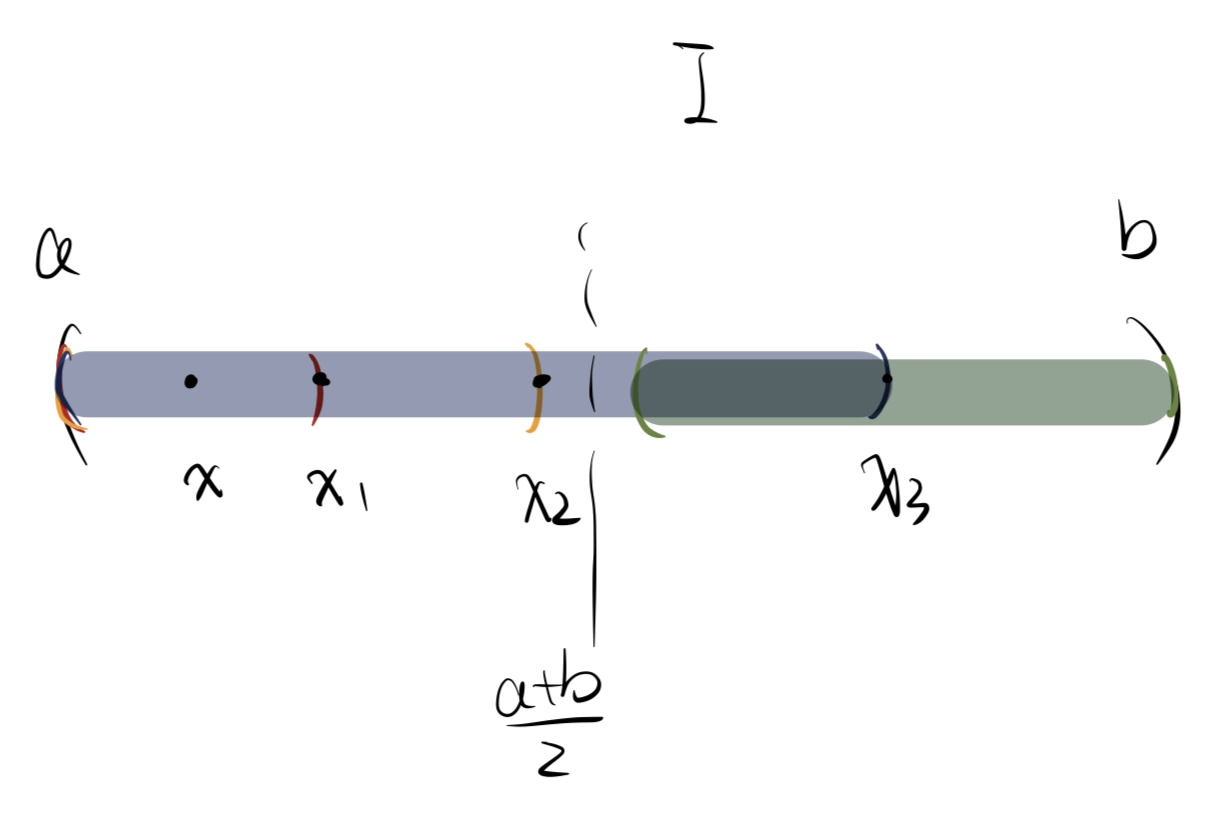
\includegraphics[width=7cm]{attachment/IMG_3538.jpg}
	\caption{\underline{\textbf{证法一}}的示意图, 手绘勿喷}
\end{figure}
	
	\underline{\textbf{证法二}}~~记$\mathcal{E}_x = \{ E \subseteq U: x \in E,E\textit{是开区间} \}$, 令$I_x = \bigcup_{E \in \mathcal{E}_x} E$. 下面证明$I_x \in \mathcal{E}_x$, 从而它就是包含$x$的最大开区间. 
	
	任取$x_1,x_2 \in I_x$, 不妨$x_1<x_2$. 由于存在分别包含$x_1,x_2$的开区间$E_{x_1}, E_{x_2}$, 所以$x_1,x_2 \in E_{x_1} \cup E_{x_2}$. 另一方面, 由于$x \in E_{x_1} \cap E_{x_2}$, $E_{x_1} \cup E_{x_2} \in \mathcal{E}_x$, 进一步$(x_1,x_2) \in \mathcal{E}_x$. 
	
	现在, 记$a = \inf I_x,b = \sup I_x$, 其中$a,b$可以是无穷. 那么对任意$c \in (a,b)$都存在$x_1,x_2$使得$a \leq x_1 < c < x_2 \leq b$, 从而$(a,b) \subseteq I_x \subseteq [a,b]$. 又$I_x$是开集, 可知$I_x = (a,b)$. 
\end{proof}

与开集相对应的概念是所谓闭集. 

\begin{definition}{$\R$上的闭集}
	设$U \subseteq \R$, 称$U$是$\R$上的一个\textit{闭集}(closed set), 如果$\R - U$是开集. 
\end{definition}

一些闭集的例子是: $\R$, $\varnothing$, 任意闭区间, 任意闭区间的交集. 对开集的命题取补集即可得到: 

\begin{proposition}{$\R$上闭集的性质}
	\vspace{-2em}
	\begin{itemize}
		\item $\R,\varnothing$是闭集; 
		\item $\bigcap_{\alpha \in A} U_{\alpha}$是闭集, 其中$U_{\alpha}$是闭集, $A$是指标集; 
		\item $\bigcup_{1 \leq i \leq n} U_i$是闭集, 其中$U_i(i=1,\cdots ,n)$是闭集. 
	\end{itemize}
\end{proposition}
\begin{remark}
	容易举出无限个闭集的并集是开集的例子: 设$I_n = [1+1/n,2-1/n]$, 则$\bigcup_{n\geq 1} I_n = (1,2)$. 
\end{remark}

关于闭集, 一个重要性质是: 

\begin{proposition}{}
	设$U \subseteq \R$, 则$U$是闭集当且仅当$U$的所有聚点都在$U$中. 
\end{proposition}
\begin{proof}
	“$\Rightarrow$”: 设$U$是闭集, 任取$U$的聚点$x$. 假设$x \notin U$, 那么$x \in \R - U$, 从而存在$\varepsilon$使得$x \in B(x,\varepsilon) \subseteq \R - U$, 矛盾. 
	
	“$\Leftarrow$”: 设$U$的任意聚点都在$U$中. 假设$\R - U$不是开集, 即存在$x \notin U$使得任意包含$x$的开球$B(x) \nsubseteq \R - U$即$B(x) \cap U \neq \varnothing$. 选取$x_n \in B(x,1/n) \cap U$可知$x_n \to x$, 矛盾. 
\end{proof}

现在我们给出一个重磅结论: 

\begin{theorem}{($\R$上)连续函数的拓扑表示}
	对于$f:\R \to \R$, $f$是连续函数当且仅当开集的原像是开集, 即对任意的$U\in \tau$, $f^{-1}(U) \in \tau$. 
\end{theorem}
\begin{remark}
	通过取补集的方法, 在此定理的基础上, 我们亦可以证明$f$是连续函数当且仅当闭集的原像是闭集. 
\end{remark}
\begin{proof}
	“$\Rightarrow$”: 任取$x_0 \in f^{-1}(U)$, 记$y_0=f(x_0)$, 存在$\varepsilon$使得对任意$y \in B(y_0,\varepsilon)$都有$y \in U$. 由于$f$连续, 对$\varepsilon$存在$\delta >0$使得对任意$x \in B(x_0,\delta)$都有$|f(x)-y_0|<\varepsilon$, 进而$f(x) \in U$, 说明$x \in f^{-1}(U)$. 
	
	“$\Leftarrow$”: 任取$x_0$, 记$y_0=f(x_0)$, 对任意的$\varepsilon >0$, $f^{-1}(B(y_0, \varepsilon))$是开集, 从而存在$\delta >0$使得$B(x_0,\delta) \subseteq f^{-1}(B(y_0, \varepsilon))$, 这就是说$f(B(x_0,\delta)) \subseteq B(y_0, \varepsilon)$. 
\end{proof}

\begin{figure}[H]
	\centering
	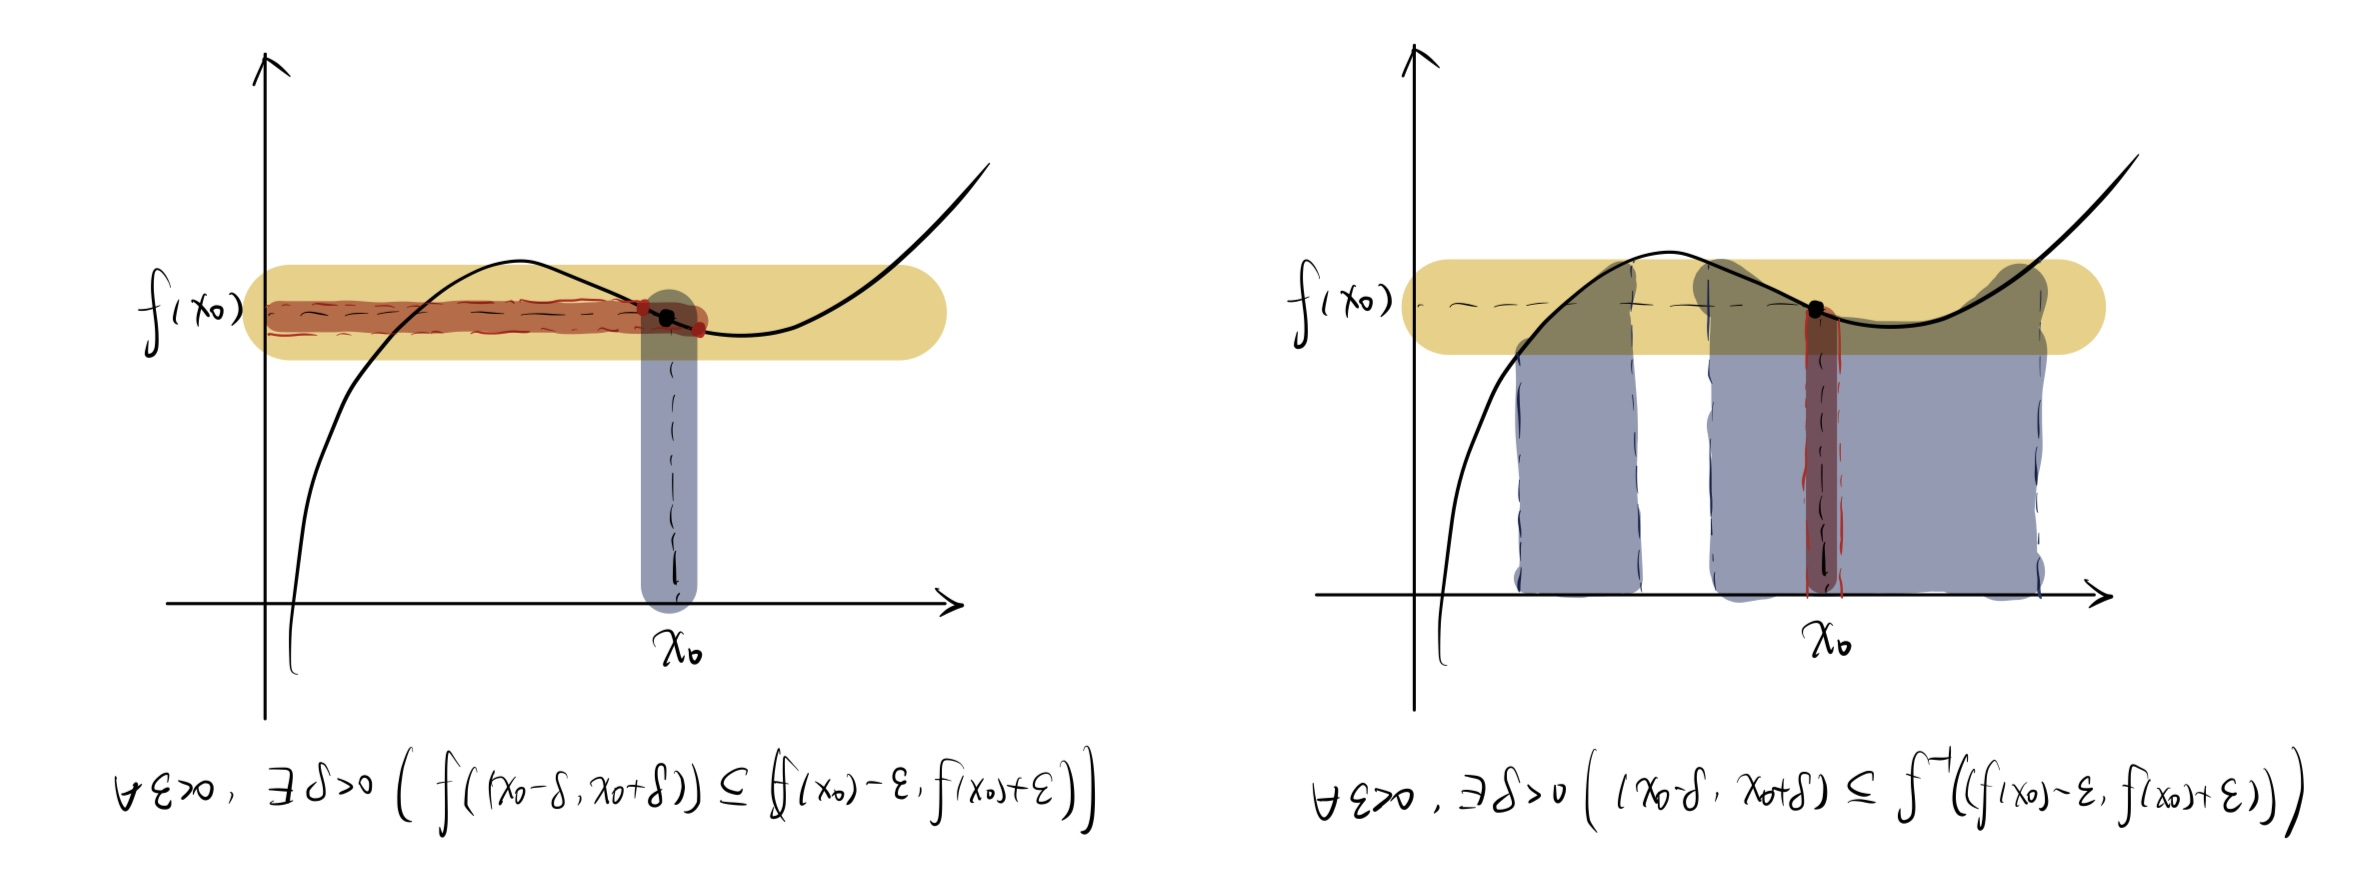
\includegraphics[width=16cm]{attachment/IMG_3539.jpg}
	\caption{两种刻画函数连续性方式的示意图, 手绘勿喷}
\end{figure}

\subsection{拓扑空间}

将开集及其性质抽象出来, 就构成一般的拓扑空间的定义. 

\begin{definition}{拓扑空间}
	设$X$为非空集合, 称$\tau \in \mathcal{P}(X)$是$X$上的一个\textit{拓扑}(topology), 如果: 
	\begin{itemize}
		\item $X \in \tau$, $\varnothing \in \tau$; 
		\item $\bigcup_{\alpha \in A} U_{\alpha} \in \tau$, 其中$U_{\alpha} \in \tau$, $A$是指标集; 
		\item $\bigcap_{1 \leq i \leq n} U_i \in \tau$, 其中$U_i \in \tau(i=1,\cdots ,n)$. 
	\end{itemize}
	接着, 称$(X,\tau)$是一个\textit{拓扑空间}(topological space), 称$\tau$中的集合为\textit{开集}(open set), 称$U \subseteq X$为\textit{闭集}(closed set)如果$X - U$是开集. 
\end{definition}

\begin{example}
	设非空集合$X$, 那么
	\begin{itemize}
		\item $\tau = \{ \varnothing ,X\}$称为$X$上的平凡拓扑, 这是$X$上最小的拓扑. 
		\item $\tau = \mathcal{P}(X)$称为$X$上的离散拓扑, 这是$X$上最大的拓扑. 
	\end{itemize}
\end{example}

类似于$\R$, 我们可以由度量自然地引出拓扑. 

\begin{proposition}{}
	设度量空间$(X,d)$, 称$U \subseteq X$是开集, 如果对任意$x \in U$都存在$\varepsilon >0$使得$B(x,\varepsilon) \subseteq U$. 那么, 由$(X,d)$上开集构成的集合是$X$上的一个拓扑. 
\end{proposition}

\begin{example}
	设非空集合$X$. 
	\begin{itemize}
		\item 拓扑空间不一定都由度量引出, 例如上面例子中的平凡拓扑. 
		\item 定义$d(x,y)= \begin{cases}
 0 &  x=y \\
 1 &  x\neq y
\end{cases}$, 则$d$引出了$X$上的离散拓扑. 
	\end{itemize}
\end{example}
\begin{proof}
	(1) 否则所有开球都要是$X$, 说明$X$上任意两点的距离可以足够小, 进而任意两点间的距离都为$0$, 不满足正定性要求. 
	
	(2) 我们先验证$d$是一个合理的距离函数, 关键在于三角不等式: 设若不然, 即存在$x,y,z \in X$使得$d(x,z)>d(x,y)+d(y,z)$, 那么必然有$d(x,z)=1,d(x,y)=d(y,z)=0$, 矛盾. 
	
	接下来证明其引出离散拓扑, 只要说明对任意$x \in X$, $\{ x \}$是开集. 注意到$\{ x \}=B(x,1/2)$即可. 
\end{proof}

现在来看看一般拓扑空间$(X,\tau)$上和开集和闭集有关的(几何的)概念. 

之前提到过, 在定义$\R$上点列的极限时, 邻域$N_{\varepsilon}(x)$的半径其实不影响最终的敛散性. 另一方面, 拓扑空间上也有可能不存在度量. 因此, 现在有必要将其一般化. 

\begin{definition}{邻域}
	设$x \in X$, 称$A \subseteq X$是$x$的一个\textit{邻域}(neighbourhood), 如果$x \in A \in \tau$. 
\end{definition}

\begin{definition}{导集, 闭包}
	设$A \subseteq X$. 
	\begin{itemize}
		\item 称$x$是$A$的一个\textit{极限点}(limited point), 如果对$x$的任意邻域$U$都有$(U \cap A) - \{ x \} = \varnothing$. 进一步, 称$A$的所有极限点组成的集合为$A$的\textit{导集}(derived set), 记作$A'$. 
		\item 称$x$是$A$的一个\textit{闭包点}(closure point), 如果对$x$的任意邻域$U$都有$U \cap A = \varnothing$. 进一步, 称$A$的所有闭包点组成的集合为$A$的\textit{闭包}(closure), 记作$\overline{A}$. 
	\end{itemize}
\end{definition}
\begin{remark}
	之前在实数章节所定义的聚点, 对应到拓扑空间上就是闭包点. (这也是为什么当时称其为聚点而不是极限点)
\end{remark}

容易证明, $A$是闭集当且仅当$A=\overline{A}$. 另外, 若$X$在$Y$中稠密, 等价地是说$\overline{X}=Y$. 

\begin{definition}{内部, 外部, 边界}
	设$A \subseteq X$. 
	\begin{itemize}
		\item 称$x$为$A$的\textit{内点}(interior point), 如果存在$x$的一个邻域是$A$的子集. 进一步, 称$A$的所有内点组成的集合为$A$的\textit{内部}(interior), 记作$\Int A$. 
		\item 称$x$为$A$的\textit{外点}(exterior point), 如果$x$是$X-A$的内点. 进一步, 称$A$的所有外点组成的集合为$A$的\textit{外部}(exterior), 记作$\Ext A$. 
		\item 称$x$为$A$的\textit{边界点}(boundary point), 如果$x$既不是$A$的内点也不是$A$的外点. 进一步, 称$A$的所有边界点组成的集合为$A$的\textit{边界}(boundary), 记作$\partial A$. 
	\end{itemize}
\end{definition}

容易证明, $A$是开集当且仅当$A= \Int A$. 另外, $\overline{A} = \Int A \cup \partial A$(这一点并不显然). 



\newpage
\section{函数列的逐点收敛与一致收敛}

\subsection{基本概念}

\subsection{度量空间$(C([a,b]),\| \bigcdot \|_{\infty})$的完备性}






























